\documentclass{article}
%\usepackage[utf8]{inputenc}
\usepackage[OT1]{fontenc} 
\usepackage[margin=0.65in]{geometry}
\usepackage{indentfirst}
\usepackage{url}
\usepackage{tikz,times}
\usetikzlibrary{mindmap}


\begin{document}
    \begin{center}
    
        \Large{Paper Review For Gene2vec} \\
        \author{}{by Anurag Banerjee}\\
        
        \vspace{1em}
        \LARGE{\textbf{Gene2vec: distributed representation of genes \\ based on co-expression}\cite{gene2vec}} \\
    	\Large{\textit{Jingcheng Du et. al.}} \\
     
    \end{center}
    \begin{normalsize}
    
    	\section{Glosssary}
		TODO
		
		\section{Problem Description}
        This paper attempts to figure out, how to represent all human \textbf{gene}s as $n$-dimensional
		vectors, such that they also capture functional relatedness of the genes.
		These vectors are to be the \textit{distributed} representation of the genes,
		in line with word embeddings (as in Natural Language Processing or NLP).
                
        \section{Problem Relevance}
        TODO
        
	   	\section{Proposed Solution}
		TODO
		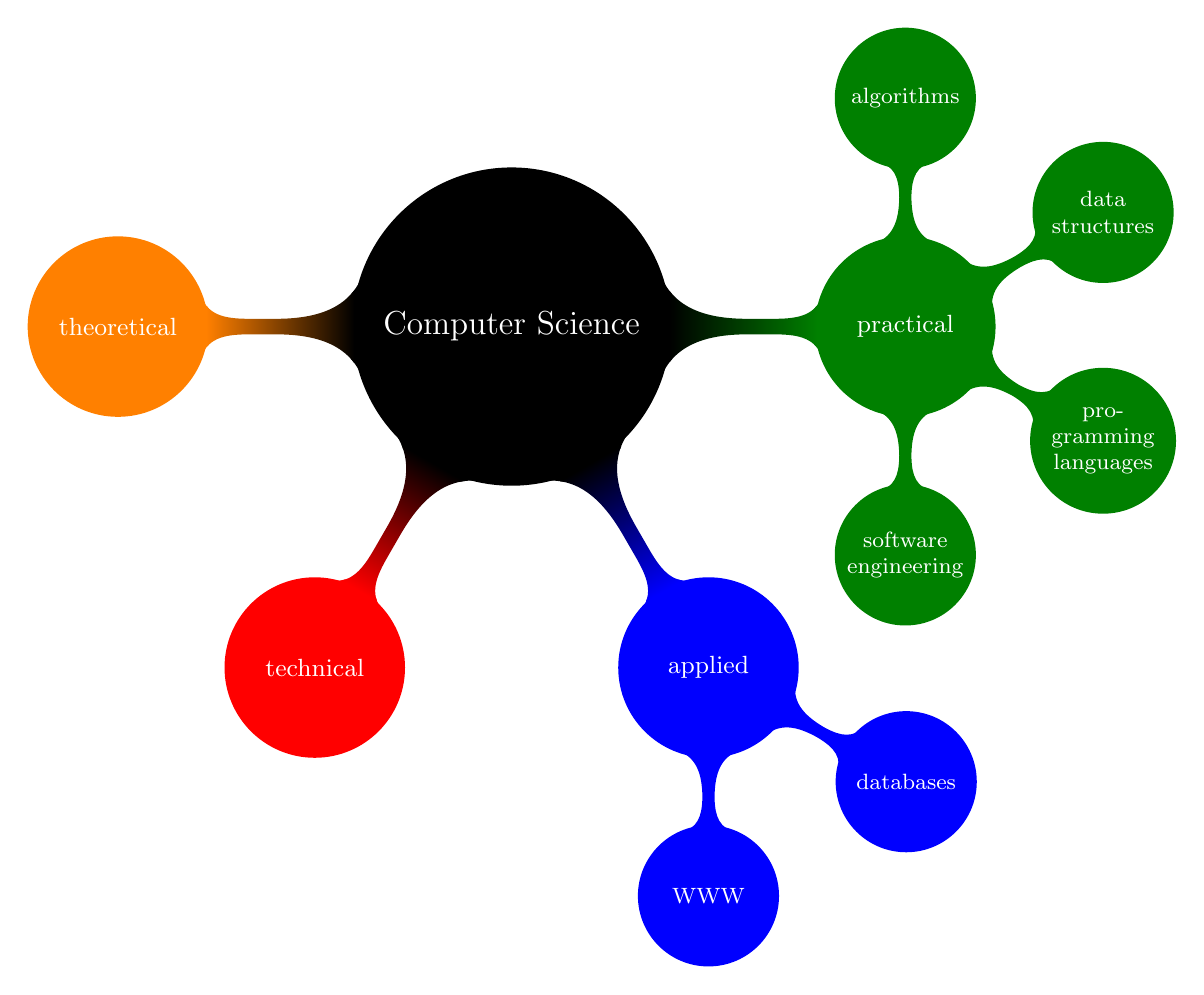
\begin{tikzpicture}
			\path[mindmap,concept color=black,text=white]
			  node[concept] {Computer Science}
			  [clockwise from=0]
			  % note that `sibling angle' can only be defined in
			  % `level 1 concept/.append style={}'
			  child[concept color=green!50!black] {
				node[concept] {practical}
				[clockwise from=90]
				child { node[concept] {algorithms} }
				child { node[concept] {data structures} }
				child { node[concept] {pro\-gramming languages} }
				child { node[concept] {software engineer\-ing} }
			  }
			  % note that the `concept color' is passed to the `child'(!)
			  child[concept color=blue] {
				node[concept] {applied}
				[clockwise from=-30]
				child { node[concept] {databases} }
				child { node[concept] {WWW} }
			  }
			  child[concept color=red] { node[concept] {technical} }
			  child[concept color=orange] { node[concept] {theoretical} };
		  \end{tikzpicture}
	   	
	   	\section{Positive Points}
	   	\begin{itemize}
	   	    \item TODO
	   	\end{itemize}
	   	
	   	\section{Negative Points}
	   	\begin{itemize}
			\item TODO
	   	\end{itemize}
	   	
	   	\section{Questions}
	   	\begin{enumerate}
	   	    \item TODO
	   	\end{enumerate}

    \end{normalsize}
    
    \bibliographystyle{ieeetr}
    \bibliography{reference}
  
\end{document}